% Тут используется класс, установленный на сервере Papeeria. На случай, если
% текст понадобится редактировать где-то в другом месте, рядом лежит файл matmex-diploma-custom.cls
% который в момент своего создания был идентичен классу, установленному на сервере.
% Для того, чтобы им воспользоваться, замените matmex-diploma на matmex-diploma-custom
% Если вы работаете исключительно в Papeeria то мы настоятельно рекомендуем пользоваться
% классом matmex-diploma, поскольку он будет автоматически обновляться по мере внесения корректив
%

% По умолчанию используется шрифт 14 размера. Если нужен 12-й шрифт, уберите опцию [14pt]
%\documentclass[14pt]{matmex-diploma}
\documentclass[14pt]{matmex-diploma-custom}

\begin{document}
\filltitle{ru}{
    chair              = {Кафедра системного программирования
          \vskip 1em
	      Программная инженерия},
    title              = {Реализация алгоритма поиска минимального остовного дерева с использованием библиотеки SuiteSparse},
    % Здесь указывается тип работы. Возможные значения:
    %   coursework - Курсовая работа
    %   diploma - Диплом специалиста
    %   master - Диплом магистра
    %   bachelor - Диплом бакалавра
    type               = {coursework},
    position           = {студента},
    group              = 271,
    author             = {Суханова Анжела Кирилловна},
    supervisorPosition = {к.\,ф.-м.\,н., доцент},
    supervisor         = {Григорьев С.\,В.},
    reviewerPosition   = {},
    reviewer           = {},
%   chairHeadPosition  = {д.\,ф.-м.\,н., профессор},
%   chairHead          = {Хунта К.\,Х.},
    university         = {Санкт-Петербургский Государственный Университет},
    faculty            = {Математико-механический факультет},
    city               = {Санкт-Петербург},
    year               = {2020}
}
\maketitle
\tableofcontents

\section*{Введение}
Графы являются одним из наиболее мощных инструментов для моделирования сложных задач благодаря своей простоте и универсальности, и алгоритмы, работающие с графами, имеют колоссальное значение в современной жизни. Анализ графструктурированных данных постепенно становится всё более популярным и находит применение в различных областях, таких как биоинформатика, анализ социальных сетей, молекулярный синтез и планирование маршрутов. В этих условиях очень важным оказывается совершенствование представлений алгоритмов на графах: в частности, поскольку графы могут содержать миллиарды вершин, возникает необходимость в распараллеливании этих алгоритмов.

К сожалению, высокопроизводительные реализации графовых алгоритмов сложно представлять на новом параллельном оборудовании (например, графических процессорах). Исследования по разработке программ для параллельного оборудования позволили ускорить графовые алгоритмы~\cite{Ligra, Gunrock}, но улучшение их производительности произошло за счёт усложнения модели программирования. В результате возникло несоответствие между языками высокого уровня, с которыми бы предпочли иметь дело пользователи и разработчики, (например, Python), и языками и стандартами программирования для параллельного оборудования (например, C$++$, CUDA, OpenMP или MPI)~\cite{GraphBLAST}. 

На устранение этой проблемы направлено несколько инициатив. Одна из них, GraphBLAS~\cite{GraphBLAS}, представляет собой открытый инновационный стандарт, определяющий структурные блоки графовых алгоритмов на языке линейной алгебры. GraphBLAS лежит в основе библиотеки, имеющей непосредственное отношение к этой работе, а именно SuiteSparse. SuiteSparse: GraphBLAS\footnote{Репозиторий с открытым исходным кодом SuiteSparse: GraphBLAS: \url{https://github.com/DrTimothyAldenDavis/SuiteSparse/tree/master/GraphBLAS} [Accessed: 31th May, 2020].}~\cite{SuiteSparse1} --- это первая полная реализация стандарта GraphBLAS (тщательно протестированная для точного соответствия спецификации), которая предоставляет множество операций над разреженными матрицами с использованием полуколец и практически неограниченного разнообразия операторов и типов. Последнее достигается за счёт того, что SuiteSparse позволяет создавать собственные типы, операторы и другие объекты и поддерживает работу с ними. Применительно к разреженным матрицам смежности эти алгебраические операции эквивалентны вычислениям на графах. Параллелизм SuiteSparse: GraphBLAS (начиная с версии 3) основан на OpenMP (GPU-версия находится в разработке)~\cite{OpenMP}.

В число графовых алгоритмов, применяемых в разных практических и теоретических областях, входит алгоритм поиска минимального остовного дерева\footnote{В этой работе вместо "минимальное остовное дерево" может быть использовано сокращение "MST" (от англ. "minimum spanning tree").}. Например, компания, желающая поставлять в несколько магазинов определённый товар с одного склада, может использовать MST для расчёта кратчайших путей к каждому фирменному магазину\footnote{В этом примере магазины и склад представлены в виде вершин (склад~--- начальная вершина), дорожные связи между ними~--- в виде рёбер, а вес каждого ребра равен длине соответствующего дорожного соединения.}. Эта работа посвящена сравнению разных решений задачи нахождения MST, основанных на линейной алгебре.


\section{Постановка задачи}
Целью данной работы является реализация алгоритма поиска минимального остовного дерева на SuiteSparse. Для её достижения были поставлены следующие задачи.

\begin{itemize}
	\item Собрать и запустить SuiteSparse, изучить её: ознакомиться с документацией по функциональности библиотеки, запустить существующие реализации и разобраться в их исходном коде.
	\item Реализовать алгоритм поиска минимального остовного дерева на SuiteSparse: GraphBLAS.
	\item Провести экспериментальное исследование реализации: осуществить замеры и анализ её производительности, сравнить их с данными исследований представлений того же алгоритма на других библиотеках высокопроизводительной обработки графов.
\end{itemize}


\section{Обзор}
\subsection{SuiteSparse: GraphBLAS}
Структуры графов на основе линейной алгебры были впервые разработаны с помощью
Combinatorial BLAS\footnote{BLAS~--- Basic Linear Algebra Subprograms (рус. базовые подпрограммы линейной алгебры).} (CombBLAS)~\cite{CombBLAS}, расширяемой библиотеки графов на основе процессоров с распределенной памятью. CombBLAS предлагает небольшой, но мощный набор примитивов линейной алгебры, предназначенный для аналитики графов. GraphBLAS, вдохновением к созданию которого послужили BLAS, основан на идее, что для реализации многих графовых алгоритмов можно использовать четыре понятия: вектор, матрицу, операцию и полукольцо~\cite{GraphBLAST}. 
\begin{itemize}
\item \textbf{Вектор}~--- подмножество вершин некоторого графа.
\item \textbf{Матрица}~--- матрица смежности некоторого графа.
\item \textbf{Операция}~--- математическая операция, определенная в спецификации GraphBLAS. Эти операции обычно действуют на матрицы и векторы, используя элементы, определенные в терминах алгебраического полукольца.
\item \textbf{Полукольцо}~--- объект, инкапсулирующий вычисления на вершинах и рёбрах графа.
\end{itemize}
SuiteSparse: GraphBLAS предоставляет набор методов для создания, извлечения и использования и освобождения представителей следующих девяти типов объектов~\cite{SuiteSparse2}:
\begin{itemize}
\item \textbf{Тип} (GrB\_Type). Библиотека поддерживает 11 встроенных типов данных (логический, знаковые и беззнаковые целые размером 8, 16, 32 и 64 бита, а также с плавающей запятой одинарной и двойной точности). 
\item \textbf{Унарный оператор} (GrB\_UnaryOp): представляет из себя функцию вида z = f(x).
\item \textbf{Бинарный оператор} (GrB\_BinaryOp): представляет из себя функцию вида z = f(x, y).
\item \textbf{Оператор выбора} (GxB\_SelectOp): используется в операции \\GxB\_select для выбора подмножества записей из матрицы.
\item \textbf{Моноид} (GrB\_Monoid)~--- это ассоциативный, коммутативный бинарный оператор z = f (x, y) (типы x, y и z одинаковы), для которого существует нейтральный элемент. Скалярное сложение при умножении матриц заменяется моноидом.
\item \textbf{Полукольцо} (GrB\_Semiring): состоит из моноида и оператора «умножения». Вместе эти операторы определяют произведение матриц C = AB, где при умножении матриц моноид используется в качестве аддитивного оператора, а оператор «умножения» полукольца~--- в качестве скалярного умножения.
\item \textbf{Дескриптор} (GrB\_Descriptor): используется для настройки параметров операций GraphBLAS.
\item \textbf{Вектор} (GrB\_Vector)~--- одномерный массив значений любого типа. $2^{60}\times 1$~--- размер cамого большого GrB\_Vector, который может быть построен. Первый элемент вектора имеет индекс 0.
\item \textbf{Матрица} (GrB\_Matrix)~--- двумерный массив значений любого типа. $2^{60}\times 2^{60}$~--- размер наибольшей GrB\_Matrix. Индексы строк и столбцов матрицы начинаются с 0.
\end{itemize}
Также пользователь может определять свои собственные типы данных, операторы, моноиды и полукольца. С полными возможностями SuiteSparse: GraphBLAS можно ознакомиться в руководстве пользователя~\cite{UserGuide}.

\subsection{Библиотеки высокопроизводительной обработки графов}
Алгоритмы поиска минимального остовного дерева были реализованы на нескольких библиотеках. В их числе:
\begin{itemize}
\item \textbf{GBTL}~\cite{GBTL} --- полная реализация спецификации GraphBLAS C API\footnote{GraphBLAS C API~--- интерфейс прикладного программирования, полностью определяющий типы, объекты, литералы и другие элементы связывания C с GraphBLAS.} на C$++$, библиотека, содержащая наиболее распространённые графовые алгоритмы, использующие GraphBLAS.
\item \textbf{LAGraph}~\cite{LAGraph} --- проект, целью которого является сбор графовых алгоритмов, построенных на основе GraphBLAS, в единую структуру.
\end{itemize}
Сравнение производительности реализации алгоритма поиска MST на SuiteSparse с существующими реализациями на вышеупомянутых библиотеках представлено в разделе \ref{1}.

Стоит отметить, что изначально планировалось представить алгоритм поиска MST на библиотеке примитивов для анализа графов на основе линейной алгебры \textbf{GraphBLAST}. GraphBLAST~\cite{GraphBLAST}--- первая реализация стандарта GraphBLAS на графическом процессоре с открытым исходным кодом\footnote{Репозиторий с открытым исходным кодом GraphBLAST: \url{https://github.com/gunrock/graphblast} [Accessed: 31th May, 2020].}, предназначенная для высокопроизводительных вычислений. Однако в ходе изучения GraphBLAST в её реализации обнаружились некоторые недочёты, о которых было сообщено разработчикам библиотеки:
\begin{itemize}
\item Не реализовано поэлементное сложение (операция eWiseAdd) разрежённых матриц и векторов. 
\item Реализация алгоритма поиска максимального независимого набора работает некорректно на всех представленных в библиотеке примерах входных графов. 
\item Конструктор матриц плохо обрабатывал графы без рёбер\footnote{К настоящему моменту эта ошибка исправлена.}.
\end{itemize}
Помимо этого многие библиотечные тесты выдают предупреждения о некорректной работе и обнаружении ошибок. В связи с этим было принято решение о переходе на SuiteSparse.

\subsection{Алгоритмы поиска минимального остовного дерева}
Поскольку нахождение MST является широко распространенной задачей в теории графов, существует много последовательных алгоритмов для ее решения. Требования к производительности решений практических проблем стали причиной распараллеливания известных алгоритмов поиска MST. В основу этой работы лёг алгоритм Борувки в силу естественности его параллельного представления и преимущества над другими алгоритмами во временной сложности в случае работы с разрежёнными графами. Это жадный алгоритм поиска минимального остовного дерева (или минимального остовного леса в случае несвязного графа). В таблице \ref{5} приведено сравнение сложности алгоритма Борувки с одним из самых известных алгоритмов поиска MST~--- алгоритмом Прима~\cite{PrimVSBoruvka}.
\begin{table}[ht]
\caption{Сравнение алгоритмов поиска MST, где n~--- количество вершин входного графа, а m~--- количество рёбер.}\label{5}
\centering
	\begin{tabular}{|c|c|c|c|}\hline
		Алгоритм & Сложность & Сложность & Критический \\
                & канонической & реализации на основе & случай (для\\
                & реализации & линейной алгебры (ЛА) & ЛА-реализации)\\\hline
		Прима & $\Theta(m+n*\log n)$ & $\Theta(n^2)$ & $\Theta(n)$ \\\hline
		Борувки & $\Theta(m*\log n)$ & $\Theta(m*\log n)$ & $\Theta(\log^2 n)$ \\\hline
	\end{tabular}
\end{table}

Кратко суть алгоритма Борувки можно изложить так:
\begin{enumerate}
\item Изначально каждая вершина графа~--- тривиальное дерево, а ребра не принадлежат никакому дереву.
\item Для каждого дерева находится минимальное инцидентное ему ребро, все такие рёбра добавляются к деревьям.
\item Второй шаг повторяется, пока в графе не останется только одно дерево. 
\end{enumerate}
Подробнее параллельная версия алгоритма Борувки описана в разделе \ref{4}.


\section{Реализация}
\subsection{Алгоритм Борувки}\label{4}
Рассмотрим псевдокод алгоритма Борувки (Input\_matrix~--- симметричная матрица смежности входного графа):
\begin{algorithmic}[1]
\Function{MST}{Input\_matrix}
\State Result $= \emptyset$
\State М $=$ Input\_matrix             
\State E $=$ \Call {Matrix\_nvals}{М}
\State N $=$ \Call {Matrix\_nrows}{М}
\State v1 $=$ \Call {Vector\_build}{[0..N-1]}
\While {$E\neq 0$}
    \State $($w, v2$) =$ \Call {Mxv}{M, v1, min, (,)}
    \ForAll {i $\in$ [0..N-1]}
    	\State v1$[$i$]$.pointer $=$ v2$[$i$]$
    \EndFor
    \ForAll {i $\in$ [0..N-1]}
        \If {v1$[$i$]$.pointer $== ($v1$[$i$]$.pointer$).$pointer}
            \State super $=$ super $\cup$ \Call {Min}{v1$[$i$]$, v1$[$i$]$.pointer}
        \EndIf
    \EndFor
    \State Result = Result $\cup$ \Call {Select}{M, select\_edge(v1, v2)}
    \State $($w, v2$) =$ \Call {Mxv}{Result, v1, min, (,)}
    \State Result $=$ \Call {Matrix\_build}{v1, v2, w} 
    \ForAll {v $\in$ super}
        \ForAll {u $\in $ \Call {сomponent}{v}}
            \State u.pointer $=$ v
        \EndFor
    \EndFor
    \State \Call {Select}{M, diff\_components()}
    \State E $=$ \Call {Matrix\_nvals}{М}
\EndWhile
\State \Return Result
\EndFunction
\end{algorithmic}

Данный алгоритм повторяет следующие фазы вычислений, итеративно добавляя выбранные рёбра в MST и удаляя некоторые рёбра из дубликата исходного графа, пока все его рёбра не будут удалены~\cite{Boruvka}:
\begin{enumerate}
\item Для каждой вершины выполняется поиск инцидентного ей ребра минимального веса. Если несколько рёбер имеют одинаковый вес, то среди них выбирается ребро с меньшим номером второй вершины. Другими словами, на первом шаге происходит выбор минимальной пары вида (вес, номер вершины), то есть исходная вершина меняет указатель на ту вершину, с которой она соединена этим ребром. Выбор ребра осуществляется посредством умножения входной матрицы на вектор номеров вершин с помощью моноида с выбором минимума в качестве бинарной операции "сложения" и конструктора пары вида (вес, номер вершины) в качестве операции "умножения" (строки 8-10).
\item Вершины и их рёбра образуют связные подграфы, каждый из которых представляет из себя два дерева, две вершины которых соединены циклом. В каждом цикле выбирается ребро, ведущее в вершину с меньшим номером (строка 13). Назовём её супервершиной, а все остальные вершины в подграфе~--- подвершинами.
\item Выбранные рёбра добавляются в MST с помощью оператора выбора (строка 14). Рёбра-дубликаты удаляются из MST(строки 15-16). Последнее осуществляется посредством умножения матрицы MST на вектор номеров вершин. 
\item Каждая подвершина находит супервершину подграфа, к которому она относится, то есть меняет указатель на неё (строки 17-19).
\item Рёбра, обе вершины которых указывают на одну и ту же супервершину, удаляются с помощью оператора выбора (строка 20).
\end{enumerate}

\subsection{Архитектура решения}
Для выполнения поставленной задачи была разработана следующая архитектура (рис. \ref{6}).

\begin{figure}
\caption{Архитектура решения}\label{6}
    \center{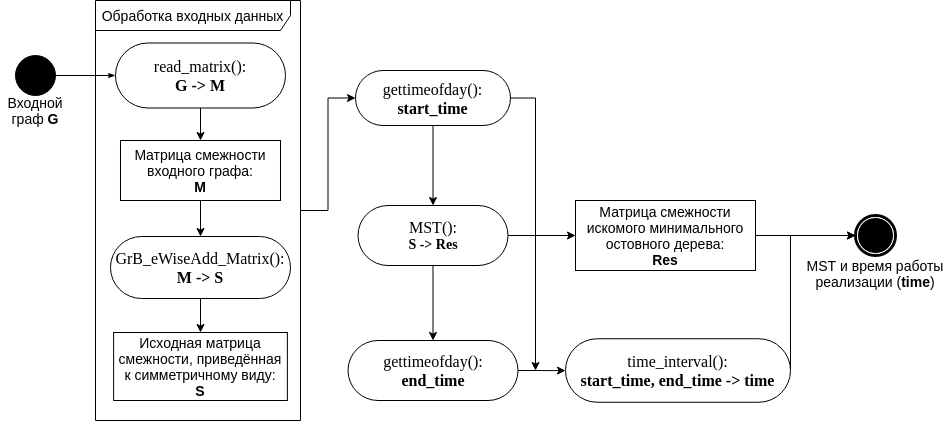
\includegraphics[width=\textwidth]{Diagram}}
\end{figure}

На вход программы подаётся файл, задающий исследуемый граф, то есть набор троек целых чисел, где первые два числа~--- номера вершин описываемого ребра, а третье число~--- вес этого ребра. Входной файл считывается функцией read\_matrix(), взятой из демо SuiteSparse\footnote{Код функции read\_matrix() можно найти здесь: \url{https://github.com/DrTimothyAldenDavis/SuiteSparse/tree/master/GraphBLAS/Demo/Source} [Accessed: 31th May, 2020].}. Функция read\_matrix() составляет матрицу смежности по заданному графу. С помощью определённой в SuiteSparse операции поэлементного сложения матриц (GrB\_eWiseAdd\_Matrix) матрица смежности приводится к симметричному виду. Важно отметить, что реализации, с которыми сравнивалась данная программа, также приводят входные матрицы к симметричному виду. Затем матрица смежности и пустая матрица для записи результата подаются в качестве параметров функции MST(), которая представляет собой реализацию алгоритма Борувки. Результат работы MST()~--- искомое минимальное остовное дерево, записанное в переданную функции пустую матрицу. Матрица с MST выводится с помощью библиотечной функции GxB\_Matrix\_fprint. Время работы функции MST() замеряется с использованием функции gettimeofday(), описанной в заголовочном файле типов и методов работы с временем sys/time.h. Достоинством этого способа измерения является большая точность ($10^{-6}$ сек). Результат замера времени поиска MST тоже выводится.

\section{Экспериментальные исследования}\label{1}
В таблице \ref{2} приведено сравнение реализации алгоритма поиска MST на SuiteSparse с реализациями на GBTL и LAGraph по времени работы. 

Таблица составлена по результатам запуска программ на тестах, отличающихся друг от друга количеством вершин, рёбер и диапазоном весов рёбер входных графов (все тесты описаны в таблице \ref{3}). Матрицы смежности графов из тестов 1-6~--- разрежённые, из тестов 7-12~--- плотные. В каждой группе тесты расположены в порядке возрастания количества вершин и рёбер для наблюдения поведения программ при увеличении нагрузки. Тесты 1, 2 и 7 запускались для исследования работы реализаций на маленьких графах. Пары тестов 3, 4 и 10, 11 имеют одинаковое количество вершин и рёбер, но разный диапазон весов рёбер, а пары 4, 5 и 8, 9, напротив, рассматриваются для изучения работы программ на графах с одинаковым диапазоном весов, но разной плотностью или количеством вершин. Тесты 6 и 12 были созданы для исследования работы реализаций на большом графе.

\begin{table}[ht]
\caption{Описание тестов.} \label{3}
\centering
	\begin{tabular}{|c|c|c|c|}\hline
		  № теста & Число рёбер & Число вершин & Диапaзон весов\\\hline
                 1 & 16 & 10 & 1 \\\hline
		 2 & 196 & 100 & 1 \\\hline
                 3 & 19996 & $10^4$ & [1, 1000] \\\hline
		 4 & 19996 & $10^4$ & [1, $10^4$] \\\hline
		 5 & 99900 & $10^4$ & [1, $10^4$] \\\hline
                 6 & 9999900 & $10^6$ & [1, $10^6$] \\\hline\hline
                 7 & 8 & 4 & 1 \\\hline
		 8 & 499500 & 1000 & [1, 5000] \\\hline
		 9 & 12497500 & 5000 & [1, 5000] \\\hline
		 10 & 40495500 & 9000 & [1, 1000] \\\hline
                 11 & 40495500 & 9000 & [1, $10^4$] \\\hline
                 12 & 49995000 & $10^4$ & [1, $10^5$] \\\hline
	\end{tabular}
\end{table}

Заметим, что замерялось только время поиска MST без учёта ввода входного графа и вывода искомого дерева. В таблице \ref{2} представлены средние значения и дисперсия по пяти запускам (в секундах). Время работы реализации алгоритма поиска MST на GBTL для тестов 6, 11 и 12 не приводится, так как на них полная работа программы (с чтением входного графа) занимает более 5 часов. Замеры проводились на ноутбуке с Ubuntu 18.04, Intel Core i5-7300HQ CPU, 2.50GHz, DDR4 64Gb RAM. 

\begin{table}[ht]
\caption{Сравнение времени работы различных реализаций (сек, число потоков: 4).} \label{2}
\centering
	\begin{tabular}{|c|c|c|c|c|c|c|}\hline
		№ & \multicolumn{2}{c|}{Данная реализация} & \multicolumn{2}{c|}{На GBTL} & \multicolumn{2}{c|}{На LAGraph}\\
		теста & Среднее & D & Среднее & D & Среднее & D \\
                & значение && значение && значение &\\\hline
		1 & 0.0013 & < 0.0001 & 0.0008 & < 0.0001 & 0.0009 & < 0.0001 \\\hline
		2 & 0.0057 & < 0.0001 & 0.0395 & < 0.0001 & 0.0011 & < 0.0001 \\\hline
        	3 & 1.0661 & 0.0001 & 131.8307 & 0.0404 & 0.0224 & 0.0001 \\\hline
        	4 & 1.0650 & 0.0002 & 132.1019 & 0.7902 & 0.0232 & < 0.0001 \\\hline
        	5 & 1.0856 & 0.0010 & 160.2648 & 1.9344 & 0.0226 & < 0.0001 \\\hline
        	6 & 160.1692 & 0.2206 &&& 2.2857 & 0.0310 \\\hline\hline
                7 & 0.0008 & < 0.0001 & 0.0002 & < 0.0001 & 0.0008 & < 0.0001 \\\hline
        	8 & 0.1303 & < 0.0001 & 19.6429 & 0.0007 & 0.0771 & < 0.0001 \\\hline
        	9 & 1.4475 & 0.0199 & 2270.5567 & 4.4393 & 1.3501 & < 0.0001 \\\hline
        	10 & 1.7971 & 0.0051 & 13090.2499 & 91.5499 & 3.8008 & 0.0007 \\\hline
        	11 & 3.5753 & 0.0052 &&& 5.2451 & 0.0010 \\\hline
        	12 & 5.7335 & 0.0002 &&& 8.0566 & 0.0045 \\\hline
        \end{tabular}
\end{table}

По таблице \ref{2} видно, что при расширении диапазона весов вершин на тестах с разрежёнными графами нагрузка на программы не увеличивается, а с плотными~--- значительно растёт. Это ожидаемое наблюдение: при увеличении диапазона весов снижается вероятность повторения весов рёбер, то есть это изменение почти не влияет на результат, если в графе мало рёбер, но для плотных матриц смежности оказывается принципиальным. Важно заметить, что на GBTL представлен алгоритм Прима, а на LAGraph~--- алгоритм Борувки, то есть реализация алгоритма Прима ощутимо отстаёт от реализаций алгоритма Борувки (хотя для совсем маленьких задач она быстрее). Представление алгоритма Борувки на LAGraph заметно обгоняет представление на SuiteSparse почти на всех тестах, но отстаёт на больших плотных графах, что может быть связано с особенностями обработки рёбер реализацией на LAGraph. 


\section*{Заключение}
В ходе выполнения данной работы были достигнуты следующие результаты:
\begin{itemize}
    \item Собрана и изучена библиотека высокопроизводительной обработки графов SuiteSparse.
    \item Реализован алгоритм поиска MST на SuiteSparse : GraphBLAS.
    \item Проведено исследование производительности реализации, в том числе сравнение с представлениями алгоритмов поиска MST на других библиотеках, основанных на GraphBLAS.
\end{itemize}
Также были осуществлены сборка библиотеки GraphBLAST и изучение существующих на ней реализаций. В ходе ознакомления с GraphBLAST обнаружились недочёты в её реализации, о которых было сообщено разработчикам библиотеки.

GraphBLAST~--- молодая библиотека, и некоторые графовые алгоритмы на ней ещё не представлены\footnote{Список алгоритмов, которые уже представлены на GraphBLAST или нуждаются в реализации: https://github.com/gunrock/graphblast/issues/2}. В их число входит алгоритм поиска минимального остовного дерева, поэтому следующие задачи могут лечь в основу дальнейших исследований:
\begin{itemize}
    \item Cовершенствование реализации.
    \item Продолжение работы с GraphBLAST и перевод реализации на неё.
\end{itemize}  

\setmonofont[Mapping=tex-text]{CMU Typewriter Text}
\bibliographystyle{ugost2008ls}
%\bibliographystyle{ieeetr}
\bibliography{diploma.bib}
\end{document}
